\chapter{Background and Related Work}
\label{ch:2}
\noindent
\section{Fundamentals and Capabilities of Mass Spectrometry}
Mass spectrometry is a core analytical technique that characterizes chemical species by converting them into gas-phase ions 
and measuring their mass-to-charge ratio ($m/z$). \cite[p.~5]{Hoffmann2011}
A mass spectrometer therefore acts as a highly sensitive "molecular balance" whose output 
-- a mass spectrum -- reports which ionic species are present and with what relative abundances. 

Conceptually, an MS experiment comprises three main steps:
\newcounter{mssteps} 
\begin{enumerate}[label=(\roman*)]
    \item \textbf{ionization}, in which neutral molecules are transferred into the gas phase and charged; \cite[p.~1]{Hoffmann2011}
    \item \textbf{mass analysis}, in which ions are separated according to $m/z$; and 
    \item \textbf{detection}, in which ion signals are recorded and assembled into a spectrum. \cite[p.~5]{Hoffmann2011}    
\end{enumerate}
 
Because many compounds form multiple ion species (e.g., adducts \cite[p.~21]{Hoffmann2011}, isotopologues \cite[p.~67]{Gross2006}, fragments), 
the measured spectrum is not a direct image of the neutral molecule 
but a structured measurement that must be interpreted in the context of the ionization and fragmentation processes used.
\cite[p.~16-18]{Hoffmann2011}

A key capability of MS is the \emph{identification of unknown compounds}. 
Even without prior knowledge of the analyte, MS provides constraints that narrow the space of possible identities. 
Accurate $m/z$ measurements can restrict candidate molecular formulas; isotope patterns 
(e.g., from $\mathrm{^{13}C}$, $\mathrm{^{37}Cl}$, $\mathrm{^{81}Br}$) 
further refine these candidates by providing diagnostic abundance ratios and characteristic spacings. \cite[p.~263]{Gross2006}
When fragmentation data are available 
-- either through tandem MS (MS/MS) or through ionization methods that induce fragmentation -- 
structural hypotheses can be tested by matching observed fragment ions and neutral losses to expected substructures. \cite[p.~225]{Gross2006}
In practice, unknown identification often combines these orthogonal cues with computational searches in spectral libraries and structure databases, 
where a measured spectrum is matched against reference spectra or predicted fragmentation patterns.
\cite[p.~8]{Scheubert2013}
For complex samples, chromatographic coupling (GC-MS or LC-MS) adds retention time as an additional dimension, \cite[p.~475]{Gross2006}
improving selectivity and reducing confounding effects from co-eluting compounds. \cite[p.~233-237]{Hoffmann2011}

MS is equally important for the \emph{quantification of known substances}, 
where the goal is to estimate analyte concentration rather than molecular identity. \cite[p.~260]{Hoffmann2011}
Quantitative MS is grounded in the relationship 
between the number of detected ions and the amount of analyte 
introduced into the instrument. \cite[p.~261 \& 265-266]{Hoffmann2011}
In idealized settings, ion signal intensity scales proportionally with concentration; 
in real measurements, this proportionality is skewed.
Consequently, reliable quantification typically relies on calibration strategies. 
\emph{External calibration} constructs a response curve from standards of known concentration, 
while \emph{internal standardization} -- often using isotopically labeled analogs -- 
compensates for variability during sample preparation, injection, and ionization. \cite[p.~264-268]{Hoffmann2011}
The outcome is a method that can measure trace concentrations across wide dynamic ranges, 
which is central in many applications.

Beyond identity and amount, MS provides a systematic route to \emph{deduce structural features of molecules}. 
Structural inference is primarily enabled by fragmentation behavior: 
when a precursor ion breaks apart, 
the resulting fragment ions reflect chemically plausible bond cleavages 
and rearrangements, thereby encoding information about
functional groups, substructures, and connectivity.  \cite[p.~i49]{Boecker2008}
Certain fragmentation pathways are characteristic  
-- for example, losses of small neutrals such as 
$\mathrm{H_2O}$, $\mathrm{NH_3}$, or $\mathrm{CO}$
can indicate the presence of hydroxyl, amino, or carbonyl functionalities, 
while specific fragment series can suggest 
alkyl chain lengths or aromatic substitution patterns. \cite[p.~504]{Gross2006} 
Importantly, structural elucidation from MS data is rarely a single-step deduction; 
rather, it is an inference problem in which multiple candidate structures 
may explain the same spectral evidence, especially for isomers. \cite[p.~53]{Vaniya2015}
As a result, modern workflows increasingly integrate MS measurements with computational 
models that generate and rank candidate structures based on spectral consistency.


\section{Principles of Mass Spectrometry}


\begin{figure}[ht]
    \centering
    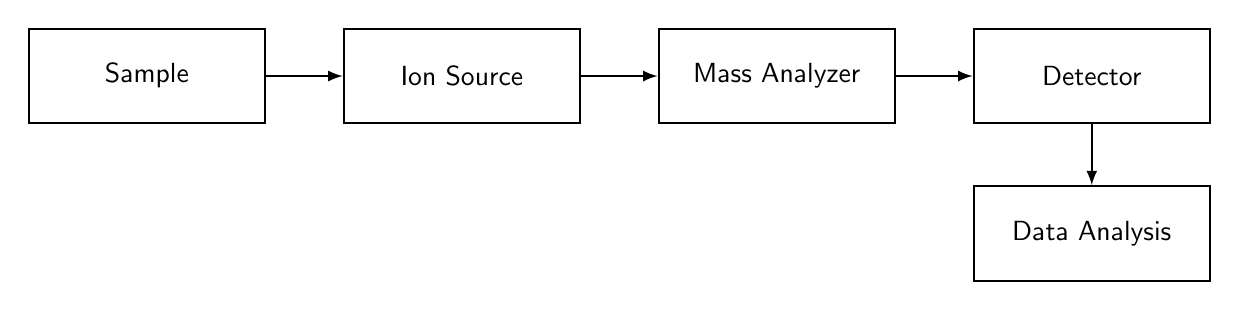
\begin{tikzpicture}[
    >=latex,
    font=\sffamily,
    block/.style={draw, thick, minimum width=3cm, minimum height=1.2cm, align=center},
    line/.style={->, thick}
    ]

% https://commons.wikimedia.org/wiki/File:Ms_block_schematic.gif


% Main horizontal blocks (fixed coordinates)
\node[block] (sample)    at (0,0)   {Sample};
\node[block] (ion)   at (4,0)   {Ion Source};
\node[block] (analyzer) at (8,0)   {Mass Analyzer};
\node[block] (det)      at (12,0)  {Detector};
\node[block] (elec) at (12,-2) {Data Analysis};

% Arrows along the ion path
\draw[line] (sample.east) -- (ion.west);
\draw[line] (ion.east) -- (analyzer.west);
\draw[line] (analyzer.east) -- (det.west);
\draw[line] (det.south)  -- (elec.north);

\end{tikzpicture}
    \caption{Flowchart of a mass spectrometer}
    \label{fig:ms-flow}
    \cite{wikibooks-ms-flowchart}
\end{figure}

\begin{figure}
    \centering
    \begin{tikzpicture}[
  >=Latex,
  font=\sffamily\scriptsize,
  every node/.style={align=center},
  lbl/.style={draw, thick, fill=white, inner sep=2.5pt},
  smalllbl/.style={draw, thick, fill=white, inner sep=2pt},
  wire/.style={thick},
  beam/.style={thick, dashed},
  arrow/.style={->, thick},
]

% https://www.chemguide.co.uk/analysis/masspec/masspec.GIF

  % vaporised sample inlet
  \draw[arrow] (-2.1,0.0) -- (-0.35,0.0);
  \node[anchor=east] at (-2.15,-0.0) {sample};

  % Ion source / acceleration tube
  \draw[wire] (-0.35,-0.35) rectangle (2.15,0.35);

  % Ionisation element
  \draw[wire] (0.15,-0.05) .. controls (0.35,0.25) and (0.55,0.25) .. (0.75,-0.05);
  \draw[wire] (0.75,-0.05) .. controls (0.55,-0.35) and (0.35,-0.35) .. (0.15,-0.05);

  % Acceleration slits
  \foreach \x in {1.10,1.35,1.60} {
    \draw[wire] (\x,-0.35) -- (\x,0.35);
  }

  % Labels
  \node[lbl] (ionlab) at (0.2,2.15) {IONISATION};
  \draw[arrow] (ionlab.south) -- (0.45,0.38);

  \node[lbl] (acclab) at (2.8,2.25) {ACCELERATION};
  \draw[arrow] (acclab.south west) -- (1.70,0.40);

  % Path points
  \coordinate (P0) at (2.15,0.0);
  \coordinate (P1) at (3.25,0.0);
  \coordinate (P2) at (5.10,-0.85);
  \coordinate (P3) at (6.95,-2.10);

  % Vacuum tube outline
  \draw[wire] (P0) -- (P1);
  \draw[wire] (P1) .. controls (4.10,0.00) and (4.70,-0.35) .. (P2)
              .. controls (5.70,-1.35) and (6.10,-1.70) .. (P3);

  \draw[wire] ($(P0)+(0,-0.25)$) -- ($(P1)+(0,-0.25)$);
  \draw[wire] ($(P1)+(0,-0.25)$) .. controls (4.05,-0.25) and (4.65,-0.60) .. ($(P2)+(0,-0.25)$)
              .. controls (5.60,-1.60) and (6.05,-1.95) .. ($(P3)+(0,-0.25)$);

    % ------------------------------------------------------------
    % Electromagnet poles: SAME Bezier as tube, but (i) shortened and (ii) symmetric
    
    \def\magGap{0.4}   % symmetric offset from centerline (tune 0.35..0.60)
    \def\magW{9pt}      % pole thickness (tune 8pt..12pt)
    
    % We draw only the "middle" of the bend by taking two points on the curve:
    % one near the start of deflection and one near the end.
    
    % Define two anchor points along the bend (tune these if needed)
    \coordinate (Mstart) at (3.2,-0.05);
    
    % Define matching control points for this shorter segment (tune slightly if needed)
    \coordinate (Mc1) at (3.9,-0.05);
    \coordinate (Mc2) at (4.3,-0.2);
    
    % Upper pole
    \draw[brown!55, line width=\magW, line cap=butt, line join=round]
      ($(Mstart)+(0,\magGap)$)
        .. controls ($(Mc1)+(0,\magGap)$) and ($(Mc2)+(0.15,\magGap)$) .. ($(P2)+(-0.05,\magGap)$);
    
    % Lower pole (perfect mirror: -\magGap)
    \draw[brown!55, line width=\magW, line cap=butt, line join=round]
      ($(Mstart)-(0,\magGap)$)
        .. controls ($(Mc1)-(0,\magGap)$) and ($(Mc2)-(-0.15,\magGap)$) .. ($(P2)-(0.1,\magGap)$);
    
    % Label + arrow
    \node[lbl] (magn) at (5.0,0.95) {ELECTROMAGNET};
    \draw[arrow] (magn.south) -- ($(P2)+(-0.9,0.9)$);
    \draw[arrow] (magn.south) -- ($(P2)+(-0.8,0.1)$);
    % ------------------------------------------------------------

    % Ion paths
    \draw[beam, green!60!black] (P0) -- (P1)
    .. controls (4.10,0.00) and (4.70,-0.35) .. (P2)
    .. controls (5.70,-1.35) and (6.10,-1.70) .. (P3);
    
    \draw[beam, blue] ($(P0)+(0,0.10)$) -- ($(P1)+(0,0.10)$)
    .. controls (4.05,0.10) and (4.65,-0.25) .. ($(P2)+(0,0.10)$)
    .. controls (5.60,-1.20) and (6.00,-1.55) .. ($(P3)+(0,0.10)$);
    
    \draw[beam, red] ($(P0)+(0,-0.10)$) -- ($(P1)+(0,-0.10)$)
    .. controls (4.15,-0.10) and (4.75,-0.45) .. ($(P2)+(0,-0.10)$)
    .. controls (5.80,-1.50) and (6.20,-1.85) .. ($(P3)+(0,-0.10)$);
    
    % DEFLECTION label
    \node[lbl] (deflab) at (3.15,-2) {DEFLECTION};
    \draw[arrow] (deflab.north) -- (4,-1);
    
    % Detector + electronics
    \draw[wire] ($(P3)+(0.1,-0.4)$) rectangle ($(P3)+(0.4,0.4)$);
    
    \node[lbl] (detlab) at (5.15,-3.65) {DETECTION};
    \draw[arrow] (detlab.north) -- ($(P3)+(0.1,-0.2)$);
    
    \node[smalllbl, minimum width=1.35cm, minimum height=0.55cm]
    (amp) at ($(P3)+(2.0,0.0)$) {amplifier \\ \& other electronics};
    
    \draw[arrow] ($(P3)+(0.45,-0.0)$) -- (amp.west);
\end{tikzpicture}
    \caption{Schematic of a mass spectrometer}
    \label{fig:ms-schematic}
    \cite{chemguide}
\end{figure}



\subsubsection{Instrument workflow}

Figure \ref{fig:ms-flow} shows steps in a mass spectrometer: 
a \emph{sample} is introduced, converted into gas-phase ions in the ion source, 
separated according to their mass-dependent motion in the \emph{mass analyzer}, 
detected in the \emph{detector}, and finally interpreted during \emph{data analysis}. 
The central observable is the mass-to-charge ratio $m/z$. 
A mass spectrum is therefore a distribution of signal intensity as a function of $m/z$, 
where the signal reflects the abundance of ions reaching the detector. \cite[p.~1566]{Murray2013}
In most practical contexts, intensities are reported as relative intensity, 
normalized such that the most intense peak equals 100\% of the base peak.  \cite[p.~1550]{Murray2013}
The x-axis is conventionally labeled with $m/z$ (mass-to-charge ratio), a dimensionless quantity.
Labeling with mass units such as \emph{daltons} (Da), amu, or unified atomic mass unit (u) is discouraged 
-- although common in practice -- as it causes confusion with multiple charged ions. \cite[p.~1516]{Murray2013}

\subsubsection{Ion notation and precursor concepts}

Ions observed in mass spectrometry are typically derived from a neutraly charged molecule $M$. 
In electron ionization (EI) a hard ionization method, removal of an electron yields the molecular ion \cite[p.~1541]{Murray2013}
-- also called the parent ion -- denoted  $[M^{+\cdot}]$, \cite[p.~1582]{Murray2013}
a radical cation carrying both a positive charge and an unpaired electron. 
More generally, the term \emph{precursor ion} refers to the ion selected for fragmentation, \cite[p.~1578]{Murray2013}
from which product ions are generated. 
In soft ionization methods like eloctrospray, ion formation is often dominated by proton transfer, 
producing a protonated molecule  $[M+H]^+$. \cite[p.~1580]{Murray2013}

\subsubsection{Peak types: isotope, fragment, and base peaks}

A measured spectrum contains several conceptually distinct peak types. 
\emph{Isotope peaks} arise from naturally occurring heavier isotopes (e.g., $^{13}\mathrm{C}$, $^{37}\mathrm{Cl}$), 
producing characteristic $M+1$, $M+2$, $\ldots$ patterns adjacent to the monoisotopic ion peak. 
\emph{Fragment peaks} arise when precursor ions undergo dissociation, 
yielding smaller product ions whose $m/z$ values and relative intensities encode structural information. 
The \emph{base peak} is the most intense peak in the spectrum \cite[p.~1524]{Murray2013} and is used for normalization; \cite[p.~1550]{Murray2013}
it is not necessarily the molecular ion and often corresponds to a particularly stable fragment. \cite[p.~2]{Moorthy2023} \cite[p.~263]{Gross2006}

\subsection{Ionization and Fragmentation}

Ionization techniques are broadly classified into two categories based on the energy imparted to the analyte: 
\emph{hard ionization} methods, which deliver high internal energy and promote extensive fragmentation, \cite[p.~1547]{Murray2013}
and \emph{soft ionization} methods, which minimize fragmentation and favor molecular ion preservation. \cite[p.~1591]{Murray2013} \cite[p.~34]{Rockwood2018}


\subsubsection{Hard Ionization methods}

\paragraph{Electron Ionization (EI)} is a hard ionization technique 
in which a stream of high-energy electrons (typically 70 eV) collides with neutral molecules in the gas phase. \cite[p.~197]{Gross2006}
The collision transfers energy to the molecule, causing the ejection of an electron and formation 
of a radical cation $[M^{+\cdot}]$ with both a positive charge and an unpaired electron. \cite[p.~194]{Gross2006}
Because the internal energy of the molecular ion typically exceeds the activation barriers for bond cleavage, 
the $[M^{+\cdot}]$ ion spontaneously fragments into smaller product ions and neutral molecules. \cite[p.~3]{Stoddard2016}
As a result, EI mass spectra are characterized by rich fragmentation patterns that reflect the molecular structure. \cite{Ashyrmamatov2025}

The deterministic nature of EI fragmentation pathways makes electron ionization particularly valuable for structural elucidation. \cite{VargasMedina2023}
Characteristic losses of small neutral species provide diagnostic clues about functional groups and connectivity. 
EI is the dominant ionization method in gas chromatography-mass spectrometry (GC-MS) and remains widely used in small-molecule analysis. \cite[p.~1]{Amirav2021}

\paragraph{Spark Ionization (SI)}, is a hard ionization technique \cite[p.~1]{Lin2024}, 
that often utilized to detect trace elements at parts-per-billion (ppb) levels. \cite[p.~428]{Ganeev2016}
It uses high-voltage up to  $100$ kV pulsed electric sparks between two electrodes to vaporize, 
atomize, and ionize conductive or semi-conductive materials. \cite[p.~428]{Ganeev2016}

\subsubsection{Soft Ionization methods}

\paragraph{Electrospray Ionization (ESI)} is a prominent soft ionization technique particularly well-suited for coupling 
with liquid chromatography (LC-MS) and for analysis of large biomolecules. \cite{Fenn1989}
In ESI, a liquid sample is converted into a fine aerosol of charged droplets 
by applying a high electric potential (typically several kilovolts) 
between a capillary needle and a counter electrode. \cite[p.~3]{Banerjee2012}
As the droplets travel toward the mass analyzer, they undergo solvent evaporation and coulombic fission, 
eventually releasing gas-phase ions into the vacuum of the spectrometer. \cite[p.~7]{Banerjee2012} \cite[p.~53]{Dass2007}

ESI ionization is exceptionally gentle, with minimal or no fragmentation in the ion source. \cite[p.~7]{Banerjee2012} 
This characteristic makes ESI ideal for determining accurate molecular weights of intact molecules. \cite[p.~211]{Dass2007}
Notably, ESI can generate multiply charged ions $[M+nH]^{n+}$ from large molecules, 
reducing their effective $m/z$ and enabling their analysis on instruments with limited mass range. \cite[p.~50]{Dass2007}

A curtain gas is often employed to shield the ion path, preventing neutral contaminants 
and solvent droplets from reaching the mass analyzer while allowing ions to pass through. \cite[p.~42]{Hoffmann2011}
The sequence from charged droplet formation to gas-phase ion release is shown in Figure~\ref{fig:esi-schematic}.


\begin{figure}[H]
    \centering
    \begin{tikzpicture}[x=1cm,y=1cm,fig]

% ---- nozzle / capillary ----
\draw[black,fig line] (0,0.35) -- (1.8,0.35) -- (2.1,0.18);
\draw[black,fig line] (0,-0.35) -- (1.8,-0.35) -- (2.1,-0.18);
\draw[black,fig line] (0,0.06) -- (2.1,0.06);
\draw[black,fig line] (0,-0.06) -- (2.1,-0.06);

% voltage probe
\draw[black,fig line] (1.25,0.35) -- (1.25,0.8);
\draw[black,fig line] (0.95,0.8) -- (1.55,0.8);
\node[above] at (1.25,0.8) {5 kV};

% labels and arrows
\node[anchor=east,align=right] at (-0.25,0.5) {Nebulizer gas};
\draw[msred,fig arrow] (-0.25,0.5) -- (0,0.18);

\node[anchor=east,align=right] at (-0.25,-0.55) {Sample solution};
\draw[msred,fig arrow] (-0.25,-0.55) -- (0,-0.25);

% ---- droplet plume: ellipse envelope + cone-shaped spray inside ----

% Linear cone (polygon): tip at left, wider to the right
\begin{scope}
  % tip and opening (tweak these 3 points if needed)
  \coordinate (tip) at (2.6,0);
  \coordinate (top) at (6.75, 0.52);
  \coordinate (bot) at (6.75,-0.52);

  \clip (tip) -- (top) -- (bot) -- cycle;

  % cone gradient (left red -> right light)
  \shade[left color=msred!85, right color=msred!5] (2.1,0.9) rectangle (7.5,-0.9);
  \shade[left color=msred!25, right color=white] (5.95,0.9) rectangle (7.5,-0.9);

  % droplets inside the cone
  \foreach \x/\y/\r in {
    3.15/0.10/0.20, 3.65/0.22/0.16, 3.75/-0.06/0.23,
    4.25/0.24/0.12, 4.75/0.18/0.10,
     5.25/0.08/0.08, 5.65/-0.05/0.07,
     5.95/0.20/0.06, 6.15/-0.15/0.06, 5.85/-0.22/0.07,
     5.25/-0.25/0.08
  }{
    \draw[msred!70,fig thin,fill=white,fill opacity=0.55]
      (\x,\y) circle [radius=\r];
  }
\end{scope}

% Outer ellipse envelope ONLY (no fill / background)
\draw[black!45,fig line] (4.7,0) ellipse [x radius=2.2, y radius=0.7];

% line from ellipse envelope to first droplet
\draw[msred,fig line] (3.2,-0.52) -- (2.1,-2.3);

% ---- desolvation / ion formation chain ----
\draw[black!70,fill=black!15,fig line] (2.1,-2.6) circle [radius=0.5cm];
\node[font=\normalsize,text=black] at (2.1,-2.6) {$+$};
\node[font=\normalsize,text=black] at (2.28,-2.42) {$+$};
\node[font=\normalsize,text=black] at (1.92,-2.42) {$+$};
\node[font=\normalsize,text=black] at (2.28,-2.78) {$+$};
\node[font=\normalsize,text=black] at (1.92,-2.78) {$+$};

\draw[msred,fig arrow] (2.75,-2.6) -- (3.8,-2.6);

\draw[black!70,fill=black!15,fig line] (4.3,-2.6) circle [radius=0.35cm];
\node[font=\small,text=black] at (4.3,-2.6) {$+$};
\node[font=\small,text=black] at (4.42,-2.48) {$+$};
\node[font=\small,text=black] at (4.18,-2.48) {$+$};
\node[font=\small,text=black] at (4.42,-2.72) {$+$};

\draw[msred,fig arrow] (4.75,-2.6) -- (5.65,-2.6);

\foreach \x/\y in {6.05/-2.8,6.45/-2.4,6.45/-3.2} {
  \node[circle,draw=black!70,fill=black!15,minimum size=0.38cm,inner sep=0pt,font=\tiny] at (\x,\y) {$+$};
}

\draw[msred,fig arrow] (6.95,-2.6) -- (8.15,-2.6);

\node[anchor=west] at (8.9,-2) {(M+H)$^{+}$};
\node[anchor=west] at (8.5,-3) {(M+H)$^{+}$};

% ---- curtain gas and mass detector ----
\node[anchor=south] at (8.2,1.1) {Curtain gas};
\draw[msred,fig arrow] (8.2,1.0) -- (8.2,0.5);

% skimmer / cone stylization (two slits with angled walls)
\draw[black!70,fig line] (8,0.8) -- (8.0,0.05);
\draw[black!70,fig line] (8,-0.3) -- (8.0,-1.0);

\draw[black!70,fig line] (8.5,0.8) -- (8.5,0.15);
\draw[black!70,fig line] (8.5,-0.3) -- (8.5,-1);
\draw[black!70,fig line] (8.5,0.15) -- (8.35,0.05);
\draw[black!70,fig line] (8.5,-0.3) -- (8.35,-0.2);

\node[anchor=west,align=left] at (9.15,0.0) {Mass detector};

\end{tikzpicture}
    \caption{Schematic of the electrospray ionization process}
    \label{fig:esi-schematic}
    \cite[p.39]{Rockwood2018}
\end{figure}

\paragraph{Atmospheric Pressure Chemical Ionization (APCI)} is a soft ionization method used primarily in LC-MS, \cite[p.~39]{Rockwood2018}
where analytes are ionized at atmospheric pressure via ion-molecule chemistry initiated by a corona discharge. \cite[p.~1522]{Murray2013}
In contrast to ESI, no high voltage is applied to the inlet capillary; 
instead, the mobile phase is nebulized, rapidly evaporated in a heated region, \cite[p.~56]{Dass2007}
and the resulting vapor passes a high-voltage needle that generates reagent ions. 
Solvents dominate the early ionization steps \cite[p.~39]{Rockwood2018} and effectively act as a reagent gas, 
transferring charge to neutral analytes mainly by proton transfer to form $[M+H]^+$.

Because APCI imparts relatively little internal energy, 
spectra typically show limited fragmentation %\cite[] 
and are well suited to quantitative LC-MS/MS, \cite[p.~171]{Dass2007} where signal is concentrated into a few precursor-ion peaks. 
A heated transfer tube and/or countercurrent curtain gas is used to 
decluster solvent-analyte adducts prior to ion extraction. \cite[p.~39]{Rockwood2018}
APCI is often more efficient than ESI for less polar compounds, \cite[p.~466]{Gross2006}
but its higher source temperatures can induce thermal degradation. \cite[p.~39]{Rockwood2018}

\begin{figure}[H]
    \centering
    \begin{tikzpicture}[x=1cm,y=1cm,>=Latex,line cap=round,line join=round,font=\sffamily]
\definecolor{msred}{RGB}{170,0,60}

% ---- nozzle / capillary (as in B: 3 lines) ----
\draw[black,line width=0.8pt] (0,0.28) -- (1.70,0.28) -- (2.05,0.12);
\draw[black,line width=0.8pt] (0,-0.28) -- (1.70,-0.28) -- (2.05,-0.12);
\draw[black,line width=0.8pt] (0,0.00) -- (2.05,0.00);

% labels + red inflow arrows
\node[anchor=east,align=right] at (-0.30,0.40) {Nebulizer gas};
\draw[msred,->,line width=0.8pt] (-0.25,0.36) -- (0,0.10);

\node[anchor=east,align=right] at (-0.30,-0.40) {Sample solution};
\draw[msred,->,line width=0.8pt] (-0.25,-0.36) -- (0,-0.10);

% ---- conical vapor/spray plume (linear) ----
\begin{scope}
  \coordinate (tip) at (2.25,0);
  \coordinate (top) at (5.90, 0.48);
  \coordinate (bot) at (5.90,-0.48);
  \clip (tip) -- (top) -- (bot) -- cycle;

  % gradient (dark near source -> light near corona region)
  \shade[left color=msred!90, right color=msred!2] (2.1,0.7) rectangle (6.4,-0.7);
\end{scope}

% ---- corona discharge region ellipse ----
\draw[black!45,line width=0.8pt] (6.50,0) ellipse [x radius=0.8cm, y radius=0.6cm];

% line form the ellipse to the flow
\draw[msred,line width=0.8pt] (5.73,-0.2) -- (0,-1.7);


\node[anchor=south] at (5.7,1) {Corona discharge};
\node[anchor=south] at (5.4,0.6) {5 kV};
\draw[black,fill=black,line width=0.2pt] (6.3,0.2) -- (6,1) -- (5.9,0.95) -- cycle;

% ---- curtain gas + interface/skimmer ----
\node[anchor=south] at (8.35,1) {Curtain gas};
\draw[msred,->,line width=0.8pt] (8.10,0.92) -- (8.10,0.35);

% skimmer / cone stylization (two slits with angled walls)
\draw[black!70,line width=0.8pt] (7.90,0.85) -- (7.90,0.10);
\draw[black!70,line width=0.8pt] (7.90,-0.25) -- (7.90,-0.95);

\draw[black!70,line width=0.8pt] (8.40,0.85) -- (8.40,0.20);
\draw[black!70,line width=0.8pt] (8.40,-0.25) -- (8.40,-0.95);
\draw[black!70,line width=0.8pt] (8.40,0.20) -- (8.25,0.10);
\draw[black!70,line width=0.8pt] (8.40,-0.25) -- (8.25,-0.15);

\node[anchor=west,align=left] at (9.20,0.00) {Mass detector};



\node at (-0.4,-2) (s1) {CH$_3$OH};
\node[below=0.02cm of s1] {M};

\node[anchor=north] at (0.9,-2.3) {5 kV};

\node at (2.5,-2) (s2) {CH$_3$OH$_2^+$};
\node[below=0.01cm of s2] {M};


% depict interaction/transfer with a small diagonal bond to M
\node at (5.5,-2) (s3) {CH$_3$OH$_2^+$};
\node[below=0.02cm of s3] (mo) {M};
\draw[black,line width=0.8pt] (5.9, -2.15) -- (5.5, -2.4);

%\node[anchor=west] at (7.25,-1.55) {(M+H)$^{+}$};-
\node[anchor=west] at (7.25,-1.95) (s4) {CH$_3$OH};
\node[below=0.02cm of s4] {(M+H)$^{+}$};


\draw[msred,->,line width=0.8pt] (s1) -- (s2);
\draw[msred,->,line width=0.8pt] (s2) -- (s3);
\draw[msred,->,line width=0.8pt] (s3) -- (s4);

\end{tikzpicture}
    \caption{Schematic of the atmospheric pressure chemical ionization process}
    \label{fig:apci-schematic}
    \cite[p.39]{Rockwood2018}
\end{figure}


\paragraph{MALDI} (Matrix-Assisted Laser Desorption/Ionization) \cite{Karas1988} is a soft ionization technique \cite{Lai2017}.
that uses a laser to desorb and ionize analytes from a solid matrix. \cite[p.~36]{Dass2007}
It is particularly effective for large biomolecules and polymers, \cite[p.~33]{Hoffmann2011}\cite[p.~36]{Dass2007} 
producing predominantly singly charged ions. \cite[p.~35]{Hoffmann2011}.
Tuning laser energy and matrix composition can optimize ionization efficiency and control fragmentation.
A general schematic of the MALDI process is shown in Figure~\ref{fig:maldi-schematic}.

\begin{figure}[H]
    \centering
    \begin{tikzpicture}[x=1cm,y=1cm,fig]

% --- small helper: red analyte ion (circle + hatch) ---
\newcommand{\analyteion}[3]{% x,y,r
  \begin{scope}[shift={(#1,#2)}]
    \draw[msred,fig line] (0,0) circle (#3);
    \draw[msred,fig thin] (-#3,-#3)--(#3,#3);
    \draw[msred,fig thin] (-#3,#3)--(#3,-#3);
    \draw[msred,fig hair] (-#3,0)--(#3,0);
    \draw[msred,fig hair] (0,-#3)--(0,#3);
  \end{scope}
}

% =========================================================
% SAMPLE STAGE (left block)
% =========================================================
\draw[black,fig medium] (0,-2.20) rectangle (0.62,1.55);

% slightly jagged "surface" line at the right edge of the stage
\draw[black,fig medium]
  (0.62,1.40) -- (0.69,1.18) -- (0.61,0.98) -- (0.70,0.78) --
  (0.62,0.58) -- (0.71,0.38) -- (0.60,0.18) -- (0.70,-0.02) --
  (0.62,-0.22) -- (0.70,-0.44) -- (0.61,-0.64) -- (0.70,-0.84) --
  (0.62,-1.04) -- (0.69,-1.26) -- (0.61,-1.46) -- (0.69,-1.68) --
  (0.62,-1.88);

% crystallized matrix bars attached to the surface
\foreach \x/\y/\rot/\w/\h in {
  0.86/ 1.30/    2/0.22/0.62,
  0.82/ 1.02/   12/0.22/0.70,
  0.90/ 0.70/  - 6/0.22/0.66,
  0.78/ 0.44/  -14/0.22/0.58,
  0.92/ 0.18/    4/0.22/0.70,
  0.80/-0.14/  -13/0.22/0.60,
  0.90/-0.46/    6/0.22/0.64,
  0.78/-0.82/    4/0.22/0.70,
  0.92/-1.18/   -4/0.22/0.62,
  0.80/-1.56/   12/0.22/0.66,
  0.92/-1.92/  -12/0.22/0.64
}{
  \begin{scope}[shift={(\x,\y)},rotate=\rot]
    \draw[black,fig line,fill=white] (-\w/2,-\h/2) rectangle (\w/2,\h/2);
  \end{scope}
}

% analyte ions embedded in the crystal pile
\analyteion{0.80}{ 1.46}{0.09}
\analyteion{0.84}{ 0.92}{0.09}
\analyteion{0.82}{ 0.36}{0.09}
\analyteion{0.80}{ 0.02}{0.09}
\analyteion{0.82}{-0.44}{0.09}
\analyteion{0.80}{-1.12}{0.09}
\analyteion{0.82}{-1.78}{0.09}

% =========================================================
% PLUME: matrix ions + neutrals (white bars), plus red analyte ions
% =========================================================
\foreach \x/\y/\rot in {
  1.30/ -0.90/  -22,
  1.45/ 0.25/  32,
  1.55/ -0.52/  10,
  1.85/ -0.30/  78,
  2.20/ 0.2/  -24,
  2.30/ -0.9/  78,
  2.65/ -0.62/  14,
  2.85/ 0.35/  -15,
  3.05/ -0.38/   6,
  3.70/ 0.70/ -18,
  3.95/ 0.92/  84,
  4.05/ -0.42/  74,
  4.30/ -0.08/  92,
  4.55/ 0.62/  14,
  4.75/ 0.30/  78,
  5.00/ 0.88/   4,
  5.20/ -0.40/  86,
  5.45/ 0.10/  92,
  5.50/ -0.74/  98,
  5.85/ 0.70/  80,
  6.10/ 1.22/  14
}{
  \begin{scope}[shift={(\x,\y)},rotate=\rot]
    \draw[black,fig medium,fill=white] (-0.11,-0.35) rectangle (0.11,0.35);
  \end{scope}
}

% analyte ions flying in the plume
\analyteion{3.65}{0.15}{0.09}
\analyteion{4.55}{-0.70}{0.09}
\analyteion{5.10}{ 0.78}{0.09}
\analyteion{5.85}{ 0.30}{0.09}
\analyteion{6.25}{-0.65}{0.09}

% =========================================================
% INCOMING UV LASER LIGHT (5 dashed rays)
% =========================================================
\foreach \dy in {-0.40,-0.20,0.00,0.20,0.40}{
  \draw[black,fig medium,dash pattern=on 4pt off 4pt]
    (1.55,0.20+\dy) -- (6.05,2.55+\dy);
}

% =========================================================
% LABELS
% =========================================================
\node[anchor=east,align=center] at (-0.35,-0.05) (sam_lab){Sample\\[-10pt]stage};
\draw[msred,->,fig medium] (sam_lab) -- (0.02,-0.55);

\node[align=center] at (2.05,-2.80) (cryst_lab) {Crystallized matrix\\[-10pt]with included analyte};
\draw[msred,->,fig medium] (cryst_lab) -- (0.92,-0.9);

\node[align=center] at (3.75,-1.60) (mat_lab) {Matrix ions and\\[-10pt]neutrals};
\draw[msred,->,fig medium] (mat_lab) -- (3.05,-0.70);
\draw[msred,->,fig medium] (mat_lab) -- (4.15,-0.59);

\node[align=center] at (6.3,-1.6) (a_lab) {Analyte\\[-10pt]ions};
\draw[msred,->,fig medium] (a_lab) -- (5.85, 0.15);
\draw[msred,->,fig medium] (a_lab) -- (6.25,-0.75);

\node[anchor=west,align=left] at (6.5,0.5) {Into mass\\[-10pt]analyzer};
\draw[msred,->,fig medium] (6.10,0.10) -- (7.95,0.10);

\node[align=center] at (2.5,2.5) (uv_lab) {Incoming UV\\[-10pt]laser light};
\draw[msred,->,fig medium] (uv_lab) -- (4.70,2.20);

\end{tikzpicture}
    \caption{
        UV laser desorbs/ionizes co-crystallized matrix and analyte, 
        creating an ion plume that is sent into the mass analyzer.
        }
    \label{fig:maldi-schematic}
    \cite[p.~42]{Rockwood2018}
\end{figure}
 
\subsection{Mass Analyzers}

After ions are generated in the ion source, they must be separated according 
to their mass-to-charge ratio $m/z$ before detection. This task is performed 
by the \textit{mass analyzer}. Mass analyzers exploit the motion of charged 
particles in electric and magnetic fields to discriminate ions with different 
$m/z$ values. The motion of an ion with mass $m$ and charge $q$ is described by 
the Lorentz force equation

\[
\left(\frac{m}{q}\right)\mathbf{a} = \mathbf{E} + \mathbf{v} \times \mathbf{B},
\]

where $\mathbf{E}$ is the electric field, $\mathbf{B}$ the magnetic field, 
$\mathbf{v}$ the ion velocity, and $\mathbf{a}$ the acceleration. 
Because ions with identical mass-to-charge ratios experience identical forces, 
they follow identical trajectories inside the analyzer. By controlling the 
fields acting on the ions, species with different $m/z$ values can therefore be 
separated before reaching the detector. \cite[p.~85]{Hoffmann2011}

Several types of mass analyzers have been developed. Among the most widely used 
are magnetic sector analyzers, time-of-flight analyzers, and quadrupole analyzers, 
each exploiting different physical principles for separating ions.

\subsubsection{Magnetic Sector Mass Analyzers}

Magnetic sector analyzers separate ions based on their deflection in a magnetic 
field. When ions enter a magnetic field perpendicular to their velocity, the 
Lorentz force bends their trajectory into a circular path. The balance between 
the magnetic force and the centripetal force yields

\[
qvB = \frac{mv^{2}}{r},
\]

where $r$ is the radius of curvature of the ion trajectory. Rearranging gives

\[
\frac{m}{q} = \frac{B^{2} r^{2}}{2V},
\]

assuming the ions were accelerated through a potential $V$. 
Thus ions with different $m/z$ values follow trajectories with different radii. 
By adjusting the magnetic field strength or the acceleration voltage, ions of 
specific mass-to-charge ratios can be selectively focused onto the detector. 
Magnetic sector instruments historically played a central role in early 
high-resolution mass spectrometry. \cite[p.~143]{Hoffmann2011}

\subsubsection{Time-of-Flight (TOF) Analyzers}

Time-of-flight analyzers separate ions based on the time required for them to 
travel a fixed distance after acceleration. When ions are accelerated through 
a potential $V$, they acquire kinetic energy

\[
\frac{1}{2}mv^{2} = qV.
\]

Solving for the velocity yields

\[
v = \sqrt{\frac{2qV}{m}}.
\]

Since ions travel through a field-free drift region of length $L$, their flight 
time $t$ is

\[
t = \frac{L}{v} = L\sqrt{\frac{m}{2qV}}.
\]

Consequently, lighter ions reach the detector earlier than heavier ones. 
Measuring the flight time therefore allows determination of the mass-to-charge 
ratio. TOF analyzers are widely used due to their fast acquisition speed and 
virtually unlimited mass range. \cite[p.~126]{Hoffmann2011}

\subsubsection{Quadrupole Analyzers}

Quadrupole analyzers consist of four parallel rods to which a combination of 
radio-frequency (RF) and direct current (DC) voltages is applied. The resulting 
oscillating electric field creates ion trajectories that are stable only for a 
specific range of mass-to-charge ratios. Ions with stable trajectories pass 
through the quadrupole and reach the detector, whereas ions with unstable 
trajectories collide with the rods and are removed. By scanning the applied 
voltages, the quadrupole sequentially transmits ions of increasing $m/z$, thereby 
producing a mass spectrum. Quadrupole analyzers are widely used in routine 
analytical instruments because of their robustness, compact design, and ability 
to operate as mass filters or in tandem mass spectrometry configurations. 
\cite[p.~88]{Hoffmann2011}

These three analyzer types illustrate the main strategies used in mass spectrometry: 
spatial separation of ion trajectories (sector instruments), 
temporal separation based on flight time (TOF), and 
stability filtering in oscillating electric fields (quadrupoles).




\subsection{Detection}

The dominant detector in EI-MS: Electron Multiplier (EM)

An electron multiplier converts a single incoming ion into a large cascade of electrons (Principle of operation):

\begin{enumerate}
    \item An ion hits the first dynode
    \item Secondary electrons are emitted
    \item These electrons are accelerated to the next dynode
    \item The process repeats (10-20 stages)
    \item Result: a measurable current pulse
\end{enumerate}

\subsection{Manual Interpretation of the MS Spectrum}

\emph{Data analysis} transforms the raw spectrum into structural hypotheses: 
isotope patterns constrain elemental composition, 
while fragment ions and neutral-loss relationships constrain functional groups and connectivity. 
Importantly, this inference is rarely a single-step deduction; 
instead, multiple candidate structures can be compatible with the same spectral evidence, particularly for isomers.

\noindent
\hrule\vspace{0.5\baselineskip}
\noindent

Here we are looking at the manuell analysis of the mass spectrum

usually well working heuristics

1. What to look for first Molecular ion peak for EI: \( [M^+ \cdot] \)

2. look for characteric isotope patterns
\begin{table}[H]
    \centering
    \caption{sample isotope patterns}
    \label{tab:placeholder_label}
    \begin{tabular}{ll}
        \hline
        Element & Diagnostic pattern \\
        \hline
        Cl & 3:1 doublet (M, M+2) \\
        Br & 1:1 doublet \\
        S & small M+2 peak \\
        C & $^{13}$C gives predictable M+1 \\
        \hline
    \end{tabular}
\end{table}

3. look for base peak (100\%) which is the energetically favored fragmentation

4. Analyze fragment differences -> look for neutral losses

5. Match fragmentation to chemical logic (reaction rules)





\subsection{Reactions in Electron Ionization}

EI reactions are well known \cite{McLafferty2013}
\section{Computational Mass Spectrometry}
\subsection{Library Search}
is a spectrum-matching procedure used to identify an unknown compound by comparing 
its measured spectrum against a reference database of known spectra.

one compares: m/z values, relative intensities

workflow: Pre-processing (Noise filtering, Peak picking, Intensity normalization, Optional deisotoping), 
Candidate filtering (precursor $\pm$ 5ppm), scoring and ranking

\subsection{In Silico Fragmentation}
predicts how a molecule will fragment in a mass spectrometer and generates a theoretical spectrum

workflow: Structure -> simulated fragments ->  predicted spectrum -> spectrum matching
\subsection{De Novo Structure Prediction}
in general:
from first principles, without relying on experimentally determined templates
in MS:
inferring the molecular structure directly from MS data, without using a reference database or known templates
\section{Graph-Based Molecular Representations}
\subsection{Molecular Graphs}
Formal definition

A molecular graph is typically defined as
\begin{equation}
    G = (V, E)
\end{equation}
where:
\begin{itemize}
    \item V ... Vertices represent atoms
    \item E ... Edges represent chemical bonds between atoms
\end{itemize}

This structure captures which atoms are connected to which, but not their explicit 3D positions unless extended.



Each node may carry attributes such as:
\begin{itemize}
    \item Element type (C, N, O, ...)
    \item Formal charge
    \item Aromaticity
    \item Hybridization
    \item Isotope
\end{itemize}


Each edge may encode:
\begin{itemize}
    \item Bond order (single, double, triple)
    \item Aromatic bond
    \item Bond stereochemistry (E/Z)
    \item Directionality (important for reactions)
\end{itemize}


By default, a molecular graph does not include:

\begin{itemize}
    \item 3D coordinates
    \item Bond lengths or angles
    \item Conformation
    \item Electronic wavefunctions
\end{itemize}
These require augmented graphs or separate geometric representations.

\subsection{Chemical Graph Transformation Systems}
reaction center (moel, coloured edges and vertecies)

\subsection{Double Pushout Graph Rewriting}

%https://www.uibk.ac.at/mathematik/algebra/staff/fritz-tobias/ct2021_course_projects/handoutdpric_fertig.pdf

morphisms


\[
    \begin{tikzcd}
    L \arrow[d, "m"'] 
    & K \arrow[l, "l"'] \arrow[r, "r"] \arrow[d] 
    & R \arrow[d, "m^{*}"] \\
    G 
    & D \arrow[l, "l^{*}"] \arrow[r, "r^{*}"'] 
    & H
    \end{tikzcd}
\]
Insertion pushout and deletion pushout
\subsection{Derivation Graph}
or Reaction Networks

describe 
\subsection{Term Mode}
Term mode is a representation mode in which chemical structures and reactions are expressed as 
formal terms (tree-like expressions) rather than as explicit graphs. 
In this mode, molecules are handled as algebraic objects governed by rewrite rules.

A term is a symbolic expression built from:

\begin{itemize}
    \item Function symbols (e.g., constructors such as C, O, bond, ring)
    \item Arguments (subterms)
\end{itemize}

Conceptually, this is similar to expressions in term-rewriting systems or functional programming.

\section{Machine Learning in Mass Spectrometry}
\subsection{Deep Learning and Spectral Embedding}
CGN GNN, featurizer vs encoder vs embedding, regularization, augmentation

MassGenie: A Transformer-Based Deep Learning Method for Identifying Small Molecules from Their Mass Spectra.
https://doi.org/10.3390/biom11121793

\section{Interpretability in Chemical Machine Learning}
